
\chapter{序論}
\label{chap:introduction}

本章ではWeb上に表示される文章レイアウトに関する現状の問題点を提示する.
それを踏まえ,本論⽂の目的,ならびに構成について述べる.

\newpage

\section{研究背景}

コンピューター技術の発展,およびスマートフォンやタブレット端末(モバイル端末)の普及に伴い,現代では
人が文章を読む媒体は活字ベースからディスプレイ上のものへと推移しつつある.
また,ブログ,SNS,チャットサービスといった文章を共有する場やコミュニケーションを行う場がインターネット上で整備されたため,
共有した文章,画像といったコンテンツが第三者に閲覧される機会,ないしリアクションをもらう相互コミュニケーションの仲介となる機会も増えた.
\\一方で,多種多様なデバイスが普及されたことにより,日本語の文章の表示には幾つかの問題が出てくる.
例えば,現在のブラウザやアプリケーションにて表示されるデザインはその画面サイズに依存した表示(レスポンシブ)デザインとなっていることによって
,その書き手側と読み手側の文章のレイアウト表示は異なる場合がある.

\begin{figure}[H]
    \centering
    \label{fig:image1}
    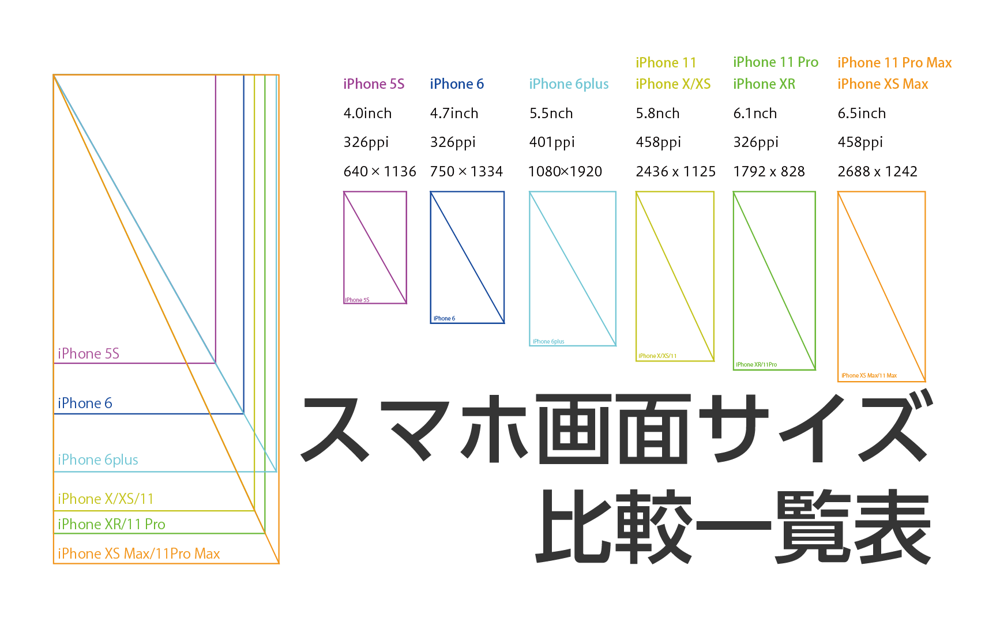
\includegraphics[width=0.7\columnwidth]{image/01/img1.png}
    \caption[スマホの画面の比較] {スマホの画面の比較\footnotemark[1]}
\end{figure}

\footnotetext[1]{
    引用元 \protect\url{
        https://developer.android.com/training/multiscreen/screensizes?hl=ja.
    }
}

例えば,PC上で書き手側が文章中に改行を加えることで,文章が横続きに長くさせないような処理を入れたとする.
それはPC上の表示では視認性の高い文章レイアウトとして表示されるが,一方で画面が縦長で表示されるスマートフォンに同じ文章を表示した
場合には意図していない箇所で改行が挟まり,視認性を損ねてしまうケースがある.
以下はslack\footnotemark[2]をPCアプリで読みやすさを意識して改行を加えた文章レイアウトをモバイルアプリにて表示した例である.


\footnotetext[2]{
    slack \protect\url{https://slack.com/intl/ja-jp/}
}
%画像がいる

\begin{figure}[H]
    \centering
    \label{fig:image5}
    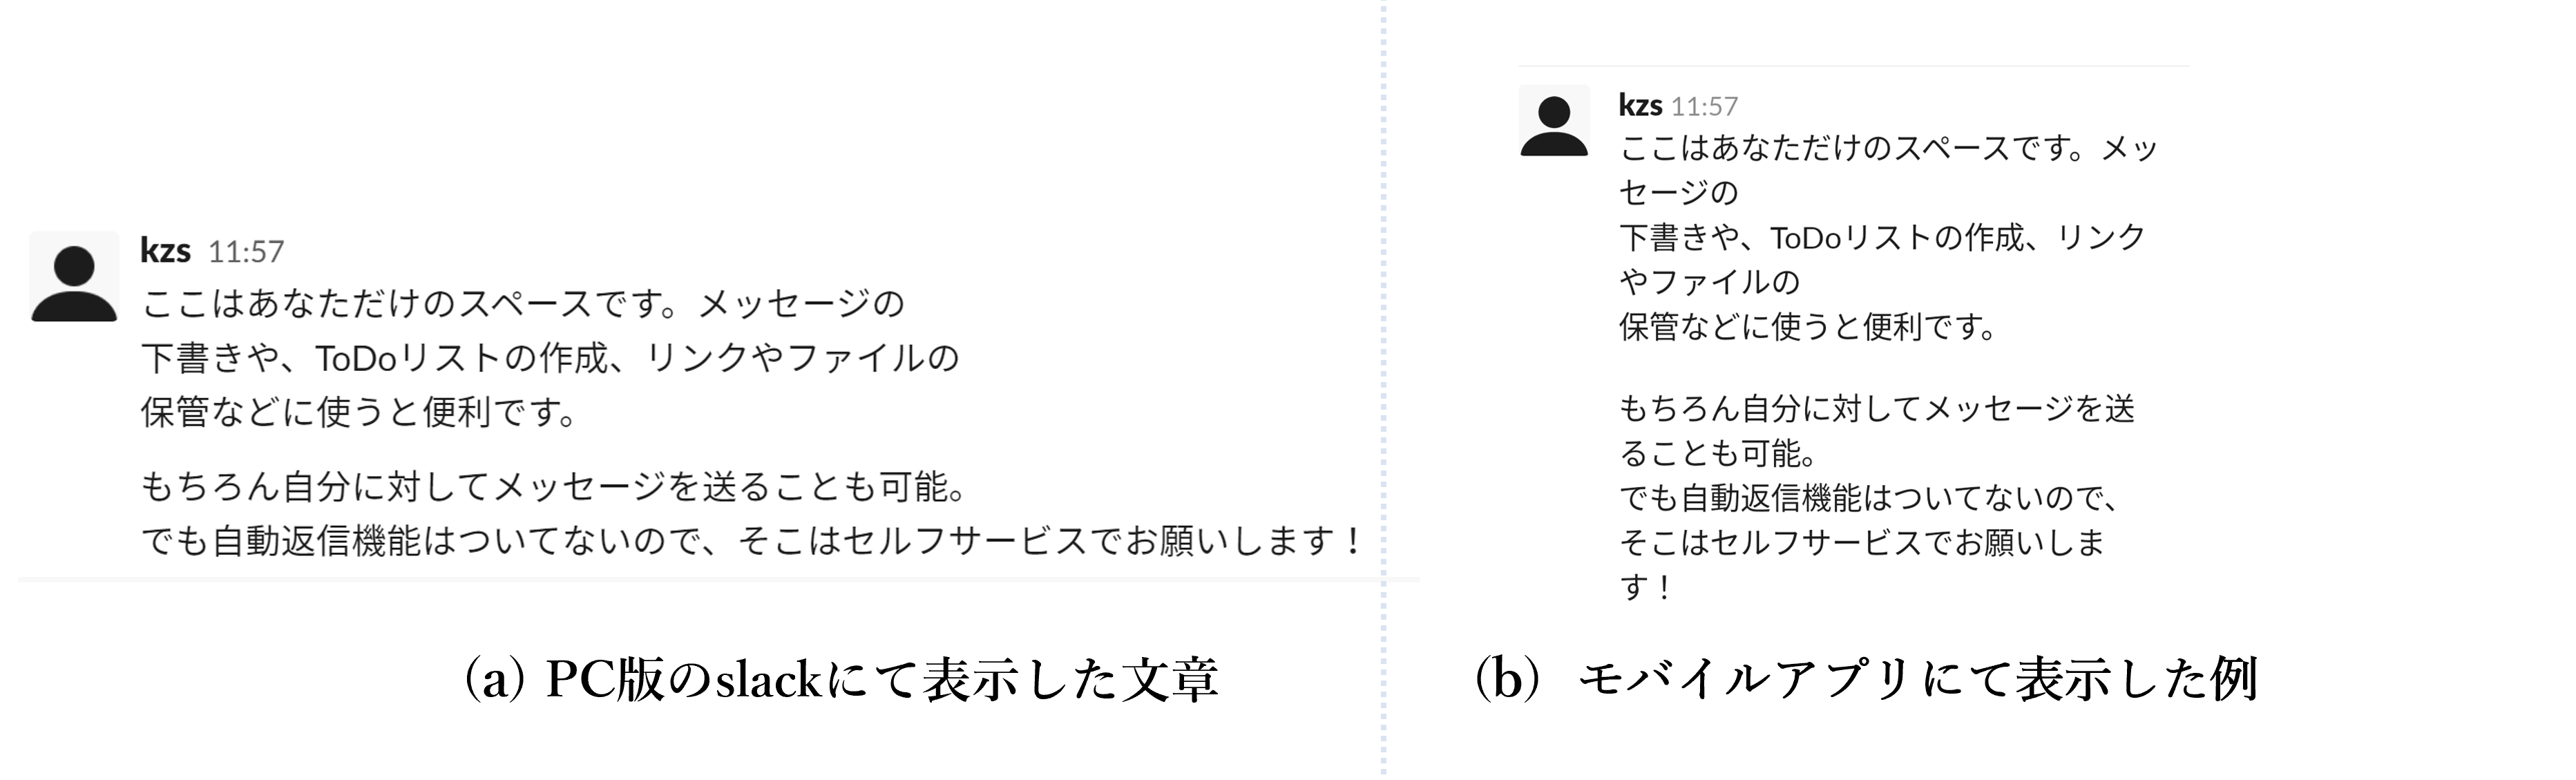
\includegraphics[width=0.9\columnwidth]{image/01/img3.png}
    \caption[PCとスマートフォンで同じ文章を表示した比較] {PCとスマートフォンで同じ文章を表示した比較}
\end{figure}

このように二者間のデバイスの違いがある中で行われる書き手の善意によって行われる文章レイアウトの編集は,
読みやすさを損ねる場合があり,結果的に読み手側のストレスとなりえる場合が発生する.
このようなケースは書き手側が自身のWYSIWYGエディタや表示環境での
視認性を高めるべく,意図的に改行を入れているため発生する.
このような文章のレイアウトの型崩れを修正することは従来の文章レンダリングでは困難であった.これを第一の問題点とする.

つづいて,文章レイアウトの問題として日本語の改行問題を取り上げる.
英語圏といった単語間をスペースで区切る言語をブラウザで表示する際,単語中に文章の折返しが挟まった場合,その単語で改行を入れる,
といった処理を自動で行なう仕様が標準的に搭載されている.一方で,日本語の文章の場合には上記のような処理は行われず,
基本は横組版のルールに基づいた両端揃えが一般的である.
このようにWeb上の日本語の文章のレイアウトには読みやすさを整える仕様は存在せず,この仕様によって読みやすさを損なうケースが存在する.
以下の画像では一行目の文末に「どこで」のいち「ど」が一文字だけが表示され,4行目の文頭で「ニャーニャー」のうち「ャー」だけが表示されるパターンも,
ひとまとまりの文意として認識しづらい表示となっている.

\begin{figure}[H]
        \centering
        \label{fig:sokoneteiru}
        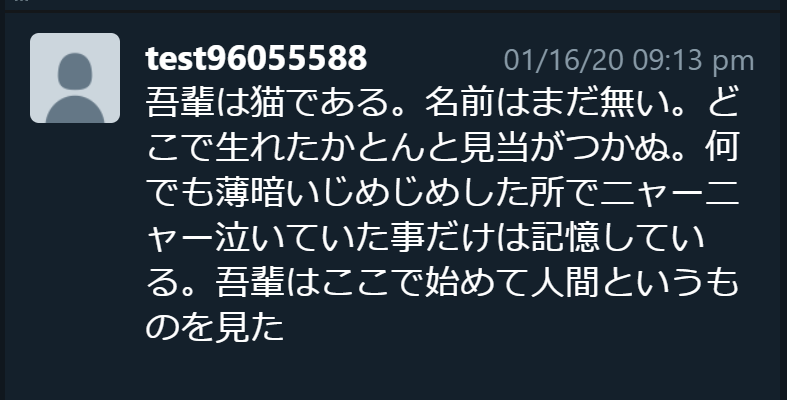
\includegraphics[width=0.7\columnwidth]{image/01/img5.png}
        \caption[ひとまとまりの文意を損ねている例] {ひとまとまりの文意を損ねている例}
\end{figure}

このように日本語の文章レイアウトには独自の問題が存在しており,これらを解消する方法は議論されてこなかった.
これを第二の問題点とした.

\section{本研究の目的}
本研究では上述した既存の日本語の文章レイアウトの問題に対して,読みづらさを解消し,
読み手側に対してリーダビリティがより高い文章レイアウトとして改稿するシステムの開発を目的とする.

\section{本論文の構成}
 本論⽂は本章を含めた6章で構成される.
 \\第2章では,本研究に関連した研究,およびライブラリを紹介した上で問題点を整理する.
 \\第3章では,本論⽂で提案するシステムの基本構成と使い⽅について述べる.
 \\第4章では,ユーザーからのフィードバックをまとめ,本論⽂で提案する
システムの有効性と問題点について述べる.
 \\最後に,第5章で本論⽂のまとめと結論を述べる.

